\documentclass[10pt,a4paper,UTF8]{ctexart}
\usepackage{geometry}%用于设置上下左右页边距
	\geometry{left=2.5cm,right=2.5cm,top=3.2cm,bottom=2.8cm}
\usepackage{xeCJK,amsmath,paralist,enumerate,booktabs,multirow,graphicx,subfig,setspace,listings,lastpage,hyperref}
\usepackage{amsthm, amssymb, bm, color, framed, graphicx, hyperref, mathrsfs}
\usepackage{mathrsfs}  
	\setlength{\parindent}{2em}
	\lstset{language=Matlab}%
\usepackage{fancyhdr}
\usepackage{graphicx}
\usepackage{listings}
\usepackage{xcolor}
\usepackage{float}

\definecolor{mKeyword}{RGB}{0,0,255}          % bule
\definecolor{mString}{RGB}{160,32,240}        % purple
\definecolor{mComment}{RGB}{34,139,34}        % green
\definecolor{mNumber}{RGB}{128,128,128} 

\lstdefinestyle {njulisting} {
	basewidth = 0.5 em,
	lineskip = 3 pt,
	basicstyle = \small\ttfamily,
	% keywordstyle = \bfseries,
	commentstyle = \itshape\color{gray}, 
	basicstyle=\small\ttfamily,
	keywordstyle={\color{mKeyword}},     % sets color for keywords
	stringstyle={\color{mString}},       % sets color for strings
	commentstyle={\color{mComment}},     % sets color for comments
	numberstyle=\tiny\color{mNumber},
	numbers = left,
	captionpos = t,
	breaklines = true,
	xleftmargin = 2 em,
	xrightmargin = 2 em,
	frame=tlrb,
	tabsize=4
}

\lstset{
style = njulisting, % 调用上述样式 
flexiblecolumns % 允许调整字符宽度
}

\pagestyle{fancy}
\lhead{\textsc{Foundation of Computing System}}
\rhead{\textsc{Nanjing University}}
\cfoot{\thepage}
\renewcommand{\headrulewidth}{0.4pt}
\renewcommand{\theenumi}{(\arabic{enumi})}


\definecolor{shadecolor}{RGB}{241, 241, 255}

\newcommand{\problemname}{待定义}
\newenvironment{problem}{\begin{shaded}\par\noindent\textbf{题目\  \problemname}}{\end{shaded}\par}
\newenvironment{solution}{\par\noindent\textbf{解答}\ }{\par}
\newenvironment{note}{\par\noindent\textbf{题目 \problemname 的注记}}{\par}

\begin{document}

\begin{center}
\LARGE\textbf{第九章习题参考答案}
\end{center}

{\kaishu 包含题目:习题$9.1-9.5$以及$9.9-9.11$}


% \begin{figure}[H]
% 	\centering
% 	\includegraphics[scale=0.3]{img/}
% \end{figure}

% \lstset{language=C}
% 	\begin{lstlisting}
	
% 	\end{lstlisting}



\renewcommand{\problemname}{9.1}
\begin{problem}
	对于DLX的I-类型指令,试回答以下问题。
	\begin{enumerate}[(1)]
		\item 立即数的范围是多少?
		\item 如果重新定义DLX的ISA,使得立即数表示无符号整数,那么,立即数的范围是多少?
		\item 如果立即数表示无符号整数,那么执行位于x3000 0000$\sim$x3000 0003中的LW指令,该指令使用R6作
			  为基址寄存器,且R6的值为x4000 0000,那么,能够加载的数据的最大地址是多少?
		\item 如果重新定义DLX的ISA,将寄存器的数量从32个降低到16个,那么,在I-类型的指令中能够表示
		的立即数的最大值是多少?假设立即数仍表示补码整数。
	\end{enumerate}
\end{problem}

\begin{solution}
	\begin{enumerate}[(1)]
		\item $-2^{15}\sim 2^{15}-1$
		\item $0\sim 2^{16}-1$
		\item 0x4000 FFFF
		\item $2^{17}-1$
	\end{enumerate}

\end{solution}


\renewcommand{\problemname}{9.2}
\begin{problem}
	对于DLX的R-类型指令,如果重新定义DLX的ISA,将寄存器的数量从32个增加至128个,是否可行?
\end{problem}

\begin{solution}
	在R-类型指令中,有5个位没有使用。
	将寄存器的数量从32个增加到128个,所需位数加2,
	总共需要位数加6,而只有5个位可用,故不可行。
\end{solution}


\renewcommand{\problemname}{9.3}
\begin{problem}
	假设某计算机的存储器包括65 536个单元,每个单元包含16位的内容,试回答以下问题。
	\begin{enumerate}[(1)]
		\item 需要多少位表示地址?
		\item 假设每条指令都由16位组成,其中一条指令与DLX无条件跳转指令(J指令)工作机制类似。如果该
		指令位于单元10中,要跳转至地址20,那么PC相对偏移量应为多少?
	\end{enumerate}

\end{problem}

\begin{solution}
	\begin{enumerate}[(1)]
		\item 16位
		\item $20-(10+1)=9$
	\end{enumerate}
\end{solution}


\renewcommand{\problemname}{9.4}
\begin{problem}
	\begin{enumerate}[(1)]
		\item 将R8乘以8,并将结果存于R9中,使用一条DLX指令能够实现吗?
	\end{enumerate}

\end{problem}

\begin{solution}
	\begin{itemize}
		\item 可以,相当于将R8左移3位后存入R9中,相应的指令为001101 01000 01001 0000000000000011
		\item 不可以,左移3位可能导致高位溢出的问题
	\end{itemize}

\end{solution}


\renewcommand{\problemname}{9.5}
\begin{problem}
	试回答下列问题:
	\begin{enumerate}[(1)]
		\item 使用一条DLX指令,可以将R1中的值移至R2中吗?
		\item 使用一条DLX指令,可以将R1中的值按位取反吗?
		\item 假设R1中存储的位组合的最右边两位有特殊的重要性,根据这两位的数值完成4个任务之一。使用
		一条DLX指令,将这两位孤立出来。
	\end{enumerate}

\end{problem}

\begin{solution}
	\begin{enumerate}[(1)]
		\item 可以,使用如下指令中的任意一条均可满足:\verb|ORI R2, R1, #0|;\ 
		\verb|ANDI  R2, R1, #-1|;\ \verb|ADDI  R2, R1, #0|;\ \verb|ADD  R2, R1, R0|
		\item 可以,指令为 \verb|XORI  r1, r1, #-1|
		\item \verb|ANDI  R1, R1, #3|
	\end{enumerate}

\end{solution}


\renewcommand{\problemname}{9.9}
\begin{problem}
	如下表所示,当一段起始于单元x3000 0000的程序执行结束后,R1$\sim$R6的值分别是多少?
\end{problem}

\begin{figure}[H]
	\centering
	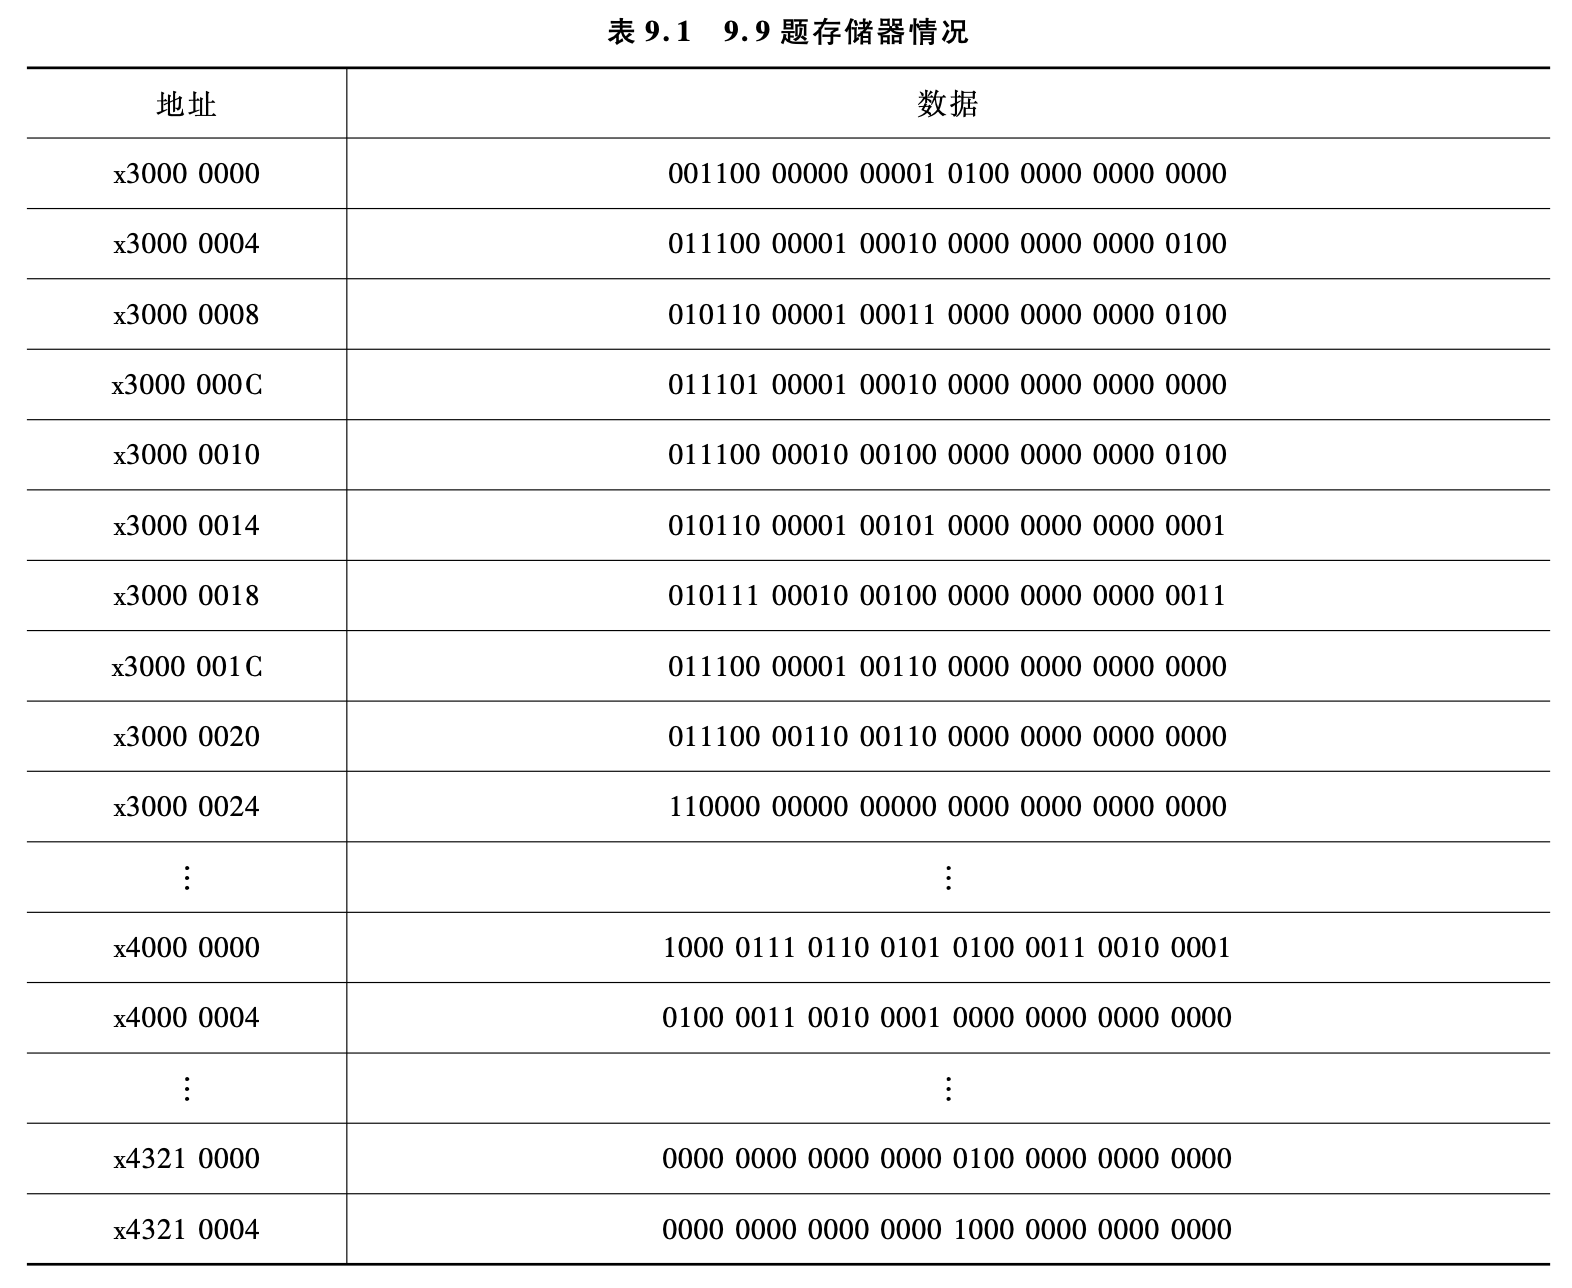
\includegraphics[scale=0.5]{img/9.9}
\end{figure}

\begin{solution}
	将机器代码翻译成汇编语言如下
	\begin{figure}[H]
		\centering
		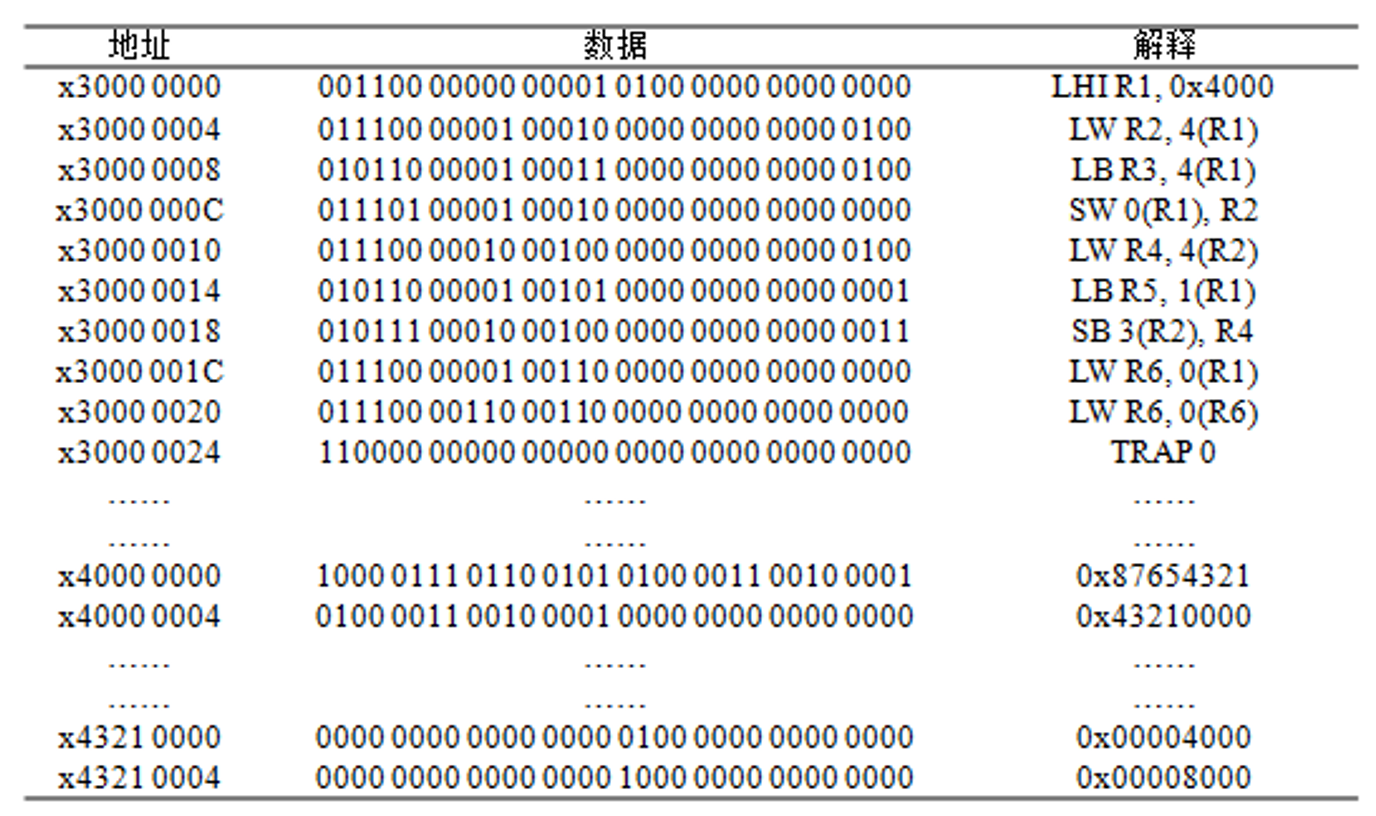
\includegraphics[scale=0.5]{img/9.9a}
	\end{figure}

	R1 = 0x4000 0000,R2 = 0x4321 0000,R3 = 0x0000 0043,
	R4 = 0x0000 8000,R5 = 0x0000 0021,R6 = 0x0000 4000。
\end{solution}


\renewcommand{\problemname}{9.10}
\begin{problem}
	下表显示了DLX存储器的一部分情况,如果条件分支将控制转移到 
	x3000 0000单元,那么R1和R2有什么特点?
\end{problem}

\begin{figure}[H]
	\centering
	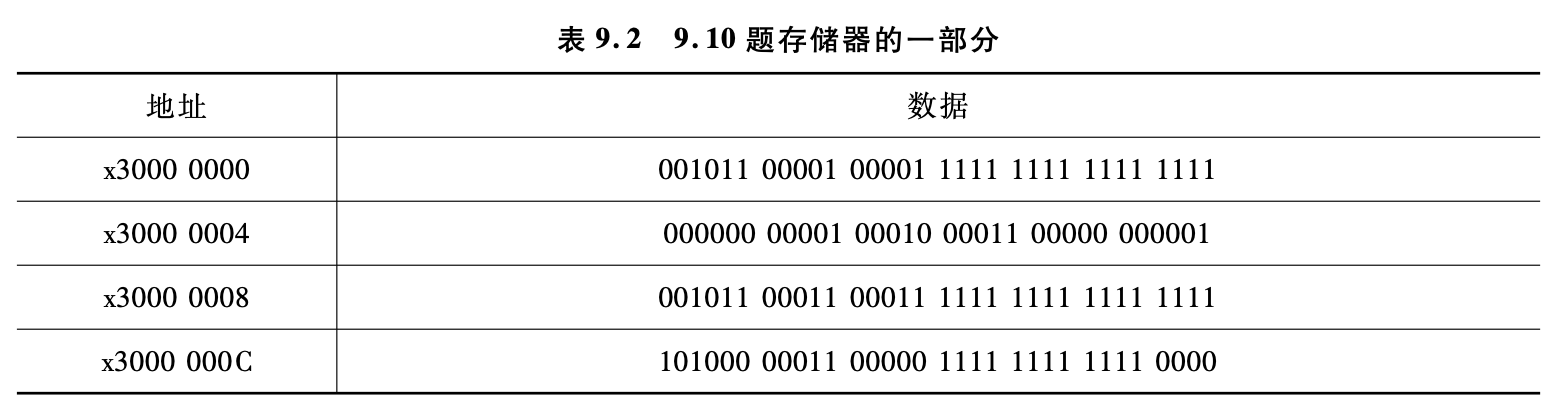
\includegraphics[scale=0.5]{img/9.10}
\end{figure}

\begin{solution}
	将机器代码翻译成汇编语言如下
	\begin{lstlisting}
XORI  r1, r1, #-1;   
ADD  r3, r1, r2;   
XORI  r3, r3, #-1; 
BEQZ  r3, 0xFFF0;
	\end{lstlisting}
	由于条件分支将控制转移到x3000 0000单元,因此 \verb|r3 = 0|,即 \verb|r3 = ~(~r1 + r2) = 0|,
	所以 \verb|~r1 + r2| \verb|= -1|,\verb|-r2 = ~r1 + 1 = ~r2 + 1|,因此有 \verb|r1 = r2|。
\end{solution}


\renewcommand{\problemname}{9.11}
\begin{problem}
	如果在下表所示的DLX指令序列执行结束时,R1中存储的值为7,由此可推知R2的什么信息?
\end{problem}

\begin{figure}[H]
	\centering
	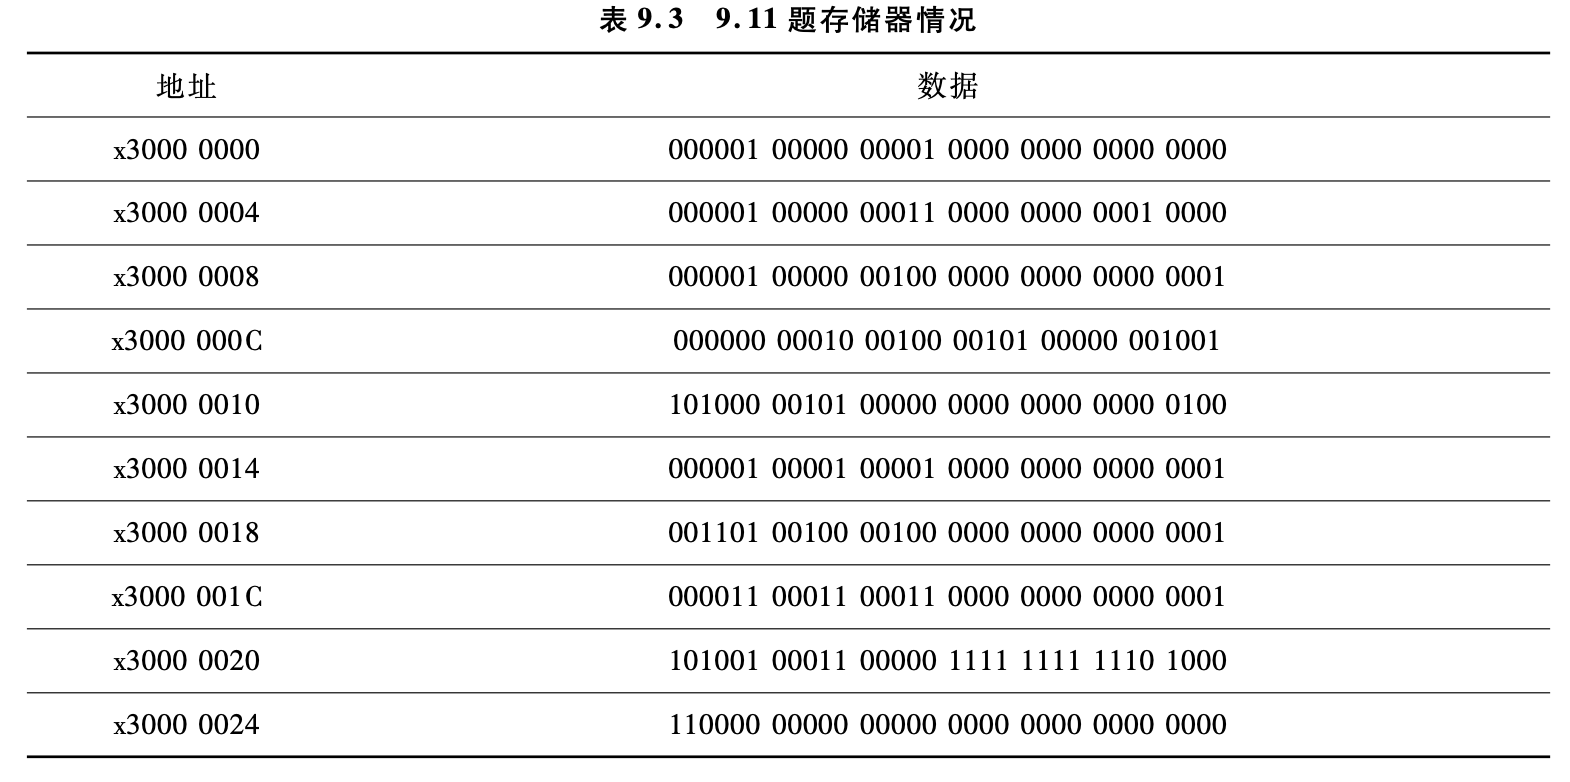
\includegraphics[scale=0.5]{img/9.11}
\end{figure}

\begin{solution}
	将机器代码翻译成汇编语言如下
	\begin{figure}[H]
		\centering
		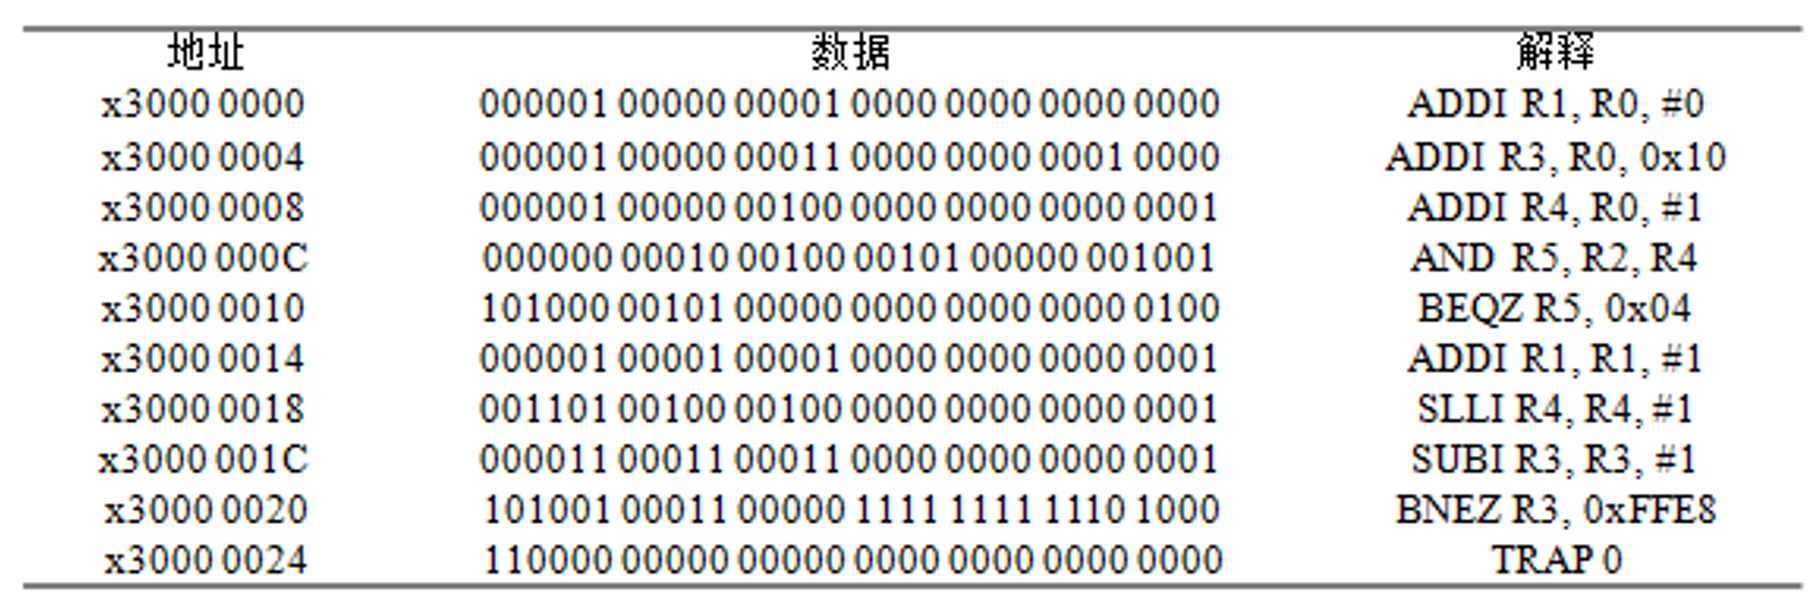
\includegraphics[scale=0.45]{img/9.11a}
	\end{figure}
	对应的C语言代码为
	\lstset{language=C}
	\begin{lstlisting}
R1 = 0;
R3 = 16;
R4 = 1;
do{
	R5 = R2 & R4;
	if (R5 != 0){
		R1 = R1 + 1;
	}
	R4 = R4 * 2;
	R3 = R3 - 1;
}while (R3 != 0);
	\end{lstlisting}

	此程序检测R2的二进制形式中1的个数。由R1为7可以知道R2的二进制形式的后16位中有7个1和$16-7=9$个0。
\end{solution}


\end{document}
